\documentclass[12pt,a4paper,reqno]{article}
\usepackage[left=12mm,top=1.5in,bottom=1.5in,right=12mm]{geometry}
\usepackage{amsmath}
\usepackage{amssymb}
\usepackage{amsmath}
\usepackage{amsthm}
\usepackage{comment}
\usepackage{tikz}
\usepackage{subcaption}
\usepackage{./slashbox}
\usepackage{enumitem}
\setlist{
  listparindent=\parindent,
  parsep=0pt,
  listparindent = 1em
}

\usetikzlibrary{matrix}

\usepackage{geometry, color, graphicx, mathtools}

\usepackage{fancyhdr}
\setlength\parindent{0pt}

\pagestyle{fancy}
\fancyhf{}
\rhead{Ria Szeredi, Kenneth Young, Lotte Romijn}
\lhead{MAST90098 Project}
\cfoot{\thepage}

\newcommand{\collie}[2]{\begin{minipage}[t]{0.20\linewidth}
{#1}
\end{minipage}
\hfill%
\begin{minipage}[t]{0.80\linewidth}
{#2}
\end{minipage}}

\renewcommand{\baselinestretch}{1.2}


\begin{document}
\title{MAST90098 \\ Approximation Algorithms and Heuristics \\ Project - 2016}
\author{Ria Szeredi, Kenneth Young, Lotte Romijn}
\maketitle


\noindent\fbox{%
    \parbox{\textwidth}{%
\textbf{Makespan Scheduling Problem (MS)} \\

Schedule $n$ jobs with designated processing times on $m$ identical machines in such a way that the whole processing time is minimised. \\

\textbf{Input}:

Positive integers $p_1,p_2,...,p_n$ and an integer $m \geq 2$ for some $n \in \mathbb{N} - \{0\}$. Each $p_i$ is the processing time of the $i$th job on any of the $m$ available machines. \\

\textbf{Constraints}:

For every input instance $(p_1,...,p_n,m)$ of MS, \\ $\mathcal{M}(p_1,...,p_n,m) = $  $\{S_1,S_2,...,S_m \> | \> S_i \subseteq \{1,2,...,n\} \textnormal{ for } i=1,...,m, \> \cup_{k=1}^m S_k = \{1,2,...,n\}, \textnormal{ and }$ \\ $S_i \cap S_j = \emptyset \textnormal{ for } i \neq j \}$. \\

\textbf{Cost}:

For each $(S_1,...,S_m) \in \mathcal{M}(p_1,...,p_n,m)$, \\ $\textnormal{cost}((S_1,...,S_m),(p_1,...,p_n,m)) = \textnormal{max} \{ \sum_{l \in S_i} p_l | i = 1,...,m \}$. \\

\textbf{Goal}:

\textit{minimum}


}
}
\newpage

\section{Greedy Local Search Algorithm for MS}
We implement a greedy local search (GLS) algorithm for MS, which picks the lowest cost neighbour at any iteration.\\

\section*{GLS 1.a}

We consider a \textit{k-jump}-neighbourhood: \\

We define a mapping $f_X: \mathcal{M}(x) \rightarrow 2^{\mathcal{M}(x)}$, such that if $\beta = \{\beta_1,\beta_2,...,\beta_m \} \in f_x(\alpha)$ for some $\alpha = \{\alpha_1,\alpha_2,...,\alpha_m \} \in \mathcal{M}(x)$ if $\beta$ can be obtained from $\alpha$ by $k$ jumps. \\

Each jump allows some job $p \in S_i$ for some $i \in \{1,...,m\}$ to move to any one of the $m$ machines, including to the one in which it is contained. Hence, after one jump we have one of two cases:
\begin{itemize}
\item $\alpha_i \neq \beta_i$ and $\alpha_j \neq \beta_j$ for some $i \in \{1,...,m\}$ and $j \in \{1,...,m\}$, and $\alpha_\ell = \beta_\ell$ for $\ell \neq i$ and $\ell \neq j$, or
\item $\alpha = \beta$ if the job jumps to its own machine. \\
\end{itemize}


We can check that the conditions for a suitable neighbourhood are satisfied. Let $\alpha = \{\alpha_1,...,\alpha_m\}$ be an initial, feasible solution.
\begin{enumerate}

\item (\textit{Reflexivity}): Since we allow a job to jump to the machine in which it is already contained, it is possible that, after $k$ jumps, all jobs are in their original machines, and the solution is identical to $\alpha$. Hence, we have that $\alpha \in f_X(\alpha)$ for every $\alpha \in \mathcal{M}(x)$. (We call this a `loop').

\item (\textit{Symmetry}): If $\beta \in f_X(\alpha)$ for some $\alpha \in \mathcal{M}(x)$, then $\alpha \in f_X(\beta)$, since reversing the $k$ jumps from which $\beta$ was obtained from $\alpha$ is also a $k$ jump.

\item (\textit{Connectivity}): If we have any two feasible solutions $\alpha$ and $\beta$, we can always obtain one from the other by performing a finite number of $k$ jumps (since we allow a job to jump to any machine). If $k \geq n$, one $k$ jump suffices, since we allow loops. If $k \leq n$, we perform maximally $\lceil \frac{n}{k} \rceil$ $k$ jumps. Hence, for all $\alpha, \beta \in \mathcal{M}(x)$, there exists a positive integer $k$ and $\gamma_1,...,\gamma_k \in \mathcal{M}(x)$ such that $\gamma_1 \in f_X(\alpha)$, $\gamma_{i+1} \in f_X(\gamma_i)$ for $i=1,...,k-1$, and $\beta \in f_X(\gamma_k)$.

\end{enumerate}

\begin{comment}
We also consider a \textit{swap}-neighbourhood: \\

We define a mapping $f_X: \mathcal{M}(x) \rightarrow 2^{\mathcal{M}(x)}$, such that if $\beta = \{\beta_1,\beta_2,...,\beta_m \} \in f_x(\alpha)$ for some $\alpha = \{\alpha_1,\alpha_2,...,\alpha_m \} \in \mathcal{M}(x)$ if $\beta$ can be obtained from $\alpha$ by $k$ swaps. \\

Each swap allows a pair of jobs $(i,j) \in \{1,...,n\} \times \{1,...,n\}$ to swap from machine.

Hence, after one swap $(\alpha_i, \alpha_j) \neq (\beta_i,\beta_j)$ for some $(i,j) \in \{1,...,n\} \times \{1,...,n\}$, and $\alpha_k = \beta_k$ for $k \neq i$ and $k \neq j$.  \\

We can check that the conditions for a suitable neighbourhood are satisfied. Let $\alpha = \{\alpha_1,...,\alpha_m\}$ be an initial, feasible solution.
\begin{enumerate}

\item (\textit{Reflexivity}): Since we allow the swapping of two jobs from the same machine, it is possible that, after a number of $k$-swaps, all jobs are in their original machines, and the solution is identical to $\alpha$. Hence, we have that $\alpha \in f_X(\alpha)$ for every $\alpha \in \mathcal{M}(x)$. (We call this a `loop').

\item (\textit{Symmetry}): If $\beta \in f_X(\alpha)$ for some $\alpha \in \mathcal{M}(x)$, then $\alpha \in f_X(\beta)$, since reversing the $k$ swap from which $\beta$ was obtained from $\alpha$ is also a $k$ swap.

\item (\textit{Connectivity}): If we have any two feasible solutions $\alpha$ and $\beta$, the connectivity property is not always satisfied. For instance, if $\alpha$ and $\beta$ only differ from each other by one job, i.e. one job is positioned into a different machine, then we can not get $\beta$ from $\alpha$ by doing one swap (or a $k$ swap, since we have reflexivity).

\end{enumerate}

Hence, for the \textit{swap}-neighbourhood the connectivity property of a neighbourhood is not satisfied. However, we can consider a neighbourhood which includes both jumps and swaps. In order to do this, we need to determine the order of jumping and swapping. For instance, a $k$-jump followed by an $l$-swap, or an $l$-swap followed by a $k$-jump, or a $k$-jump followed by an $l$-swap followed by an $s$-jump, etc., for positive integers $k$, $l$, $s$. Because such neighbourhoods include the $k$-jump neighbourhood, for which connectivity is satisfied, we have that connectivity is also satisfied for any of these combinations.
\end{comment}


\section*{GLS 1.b}
We implement the \textit{greedy local search} (GLS) algorithm in Python. We will call the resulting total processing time, produced by the algorithm, the `makespan value'. See attached \color{red} code files \color{black}. \\

In our code for GLS, Variable-Depth Search (Section \ref{}) and Simulated Annealing (Section \ref{}), we represent a feasible solution $\{S_1,S_2,...,S_m\}$ to the Makespan Scheduling problem as a list $\xi = [\xi_1,\xi_2,...,\xi_n]$ of length $n$, where each $\xi_i \in [1,...,m]$ which represents in which machine job $i$ is contained. Methods have been included which convert the solutions between these two representations (\textit{convertSol\_toListOfMachines} and \textit{convertSol\_toSetsOfJobs}). Further details about the implementation of the procedure to find the best $k$-\emph{jump}-neighbour of a solution are provided in Section \ref{}.\\

\section*{GLS 1.c}
We perform an experimental study on randomly generated instances of MS across a range of $n$ and $m$ values in order to select an appropriate value for $k$. \\

We consider $n=15, 20, 25, 30, 35, 40, 45, 50$, $m=2,4,6,8,10$, and $k=1,2,3$. For each combination of $n$, $m$ and $k$, we generate 1 instance of MS. For each instance, we randomly select the processing times $p_i$, for $i=1,...,n$, uniformly distributed between 1 and 100. We determine the runtime of our GLS implementation for each instance, and the solution quality by comparing the makespan value to a lower bound. We define this lower bound to be the least possible makespan value if we were able to process fractions of the jobs on any machine, i.e.
\begin{equation}
\textnormal{lower bound} = \frac{\sum_{i=1}^n p_i}{m}.
\end{equation}
We subsequently calculate the solution quality, denoting the makespan value produced by GLS as `makespan',
\begin{equation}
\textnormal{`makespan gap'} = \frac{\textnormal{makespan}}{\textnormal{lower bound} - 1} \times 100\%,
\end{equation}
which represents the percentage that makespan value is above its lower bound

The results of 1 realization per $n$, $m$, and $k$ are given in Table \ref{tab:Q1c} and Figure \ref{fig:Q1c}.
In Figure \ref{fig:Q1c}, we show three-dimensional plots of $n$ versus $m$ versus the makespan gap (in percentage), in Figure \ref{fig:Q1cSFig1}, \ref{fig:Q1cSFig3}, and \ref{fig:Q1cSFig5}, and $n$ versus $m$ versus the run time (in seconds), in Figure \ref{fig:Q1cSFig2}, \ref{fig:Q1cSFig4}, and \ref{fig:Q1cSFig6}. For clarity, we only plot values for the makespan between 0 and 20 \%, and values for the run time between 0 and 300 seconds. We consider a `reasonable' runtime to be approximately 5 minutes (300 seconds). \\

We can see in Table \ref{tab:Q1ck=1makespangap}, \ref{tab:Q1ck=2makespangap}, and \ref{tab:Q1ck=3makespangap} that for all $n$ and $m$, the makespan gap decreases as we increase $k$. For $k=1$, the average makespan gap for all $n$ and $m$ in Table \ref{tab:Q1ck=1makespangap} is 6.98 \%. For $k=2$,  the average makespan gap for all $n$ and $m$ in Table \ref{tab:Q1ck=2makespangap} is 3.68 \%. For $k=3$,  the average makespan gap for all $n$ and $m$ in Table \ref{tab:Q1ck=3makespangap} is 1.32 \%. The makespan gap is larger for small $n$ and large $m$, i.e. when few jobs need to be distributed over many machines. It is especially larger when $n$ is close to $m$. \color{red} SAY WHY \color{black} \\

In Table  \ref{tab:Q1ck=1runtime}, \ref{tab:Q1ck=2runtime}, and \ref{tab:Q1ck=3runtime}, we see that for all $n$ and $m$, the run time increases as $k$ increases. It increases exponentially: we see that the average run time is 0.072 s for $k=1$, 19.79 s for $k=2$, and 1199 s for $k=3$. The runtime is larger for large $m$ and large $n$, as in this case there are many possibilities for jobs to make a jump, and hence, we have a large neighbourhood. \\

For our remaining experiments, we choose $k=2$. In Figure \ref{fig:Q1cSFig4}, we see that for all instances we have considered so far, the run time is smaller than 5 minutes (300 seconds). Moreover, the makespan gap is smaller than for $k=1$, for all instances except for $n=15$ and $m=8,10$, i.e. when the number of jobs is relatively close to the number of machines. Hence, we make a trade-off between solution quality and run time, and select $k=2$ as our $k$-value.


\begin{table}
\begin{center}
{\large \bf GLS experiments with random initial solution}
\end{center}
\begin{center}
{\large \bf $k=1$}
\end{center}
\centering
\begin{subtable}{0.48\textwidth}
\centering
\caption[Makespan gap]{Makespan gap}
%\renewcommand\arraystretch{1.3}
\renewcommand\tabcolsep{1pt}
\centering
\footnotesize
\begin{tabular}{l|*{9}{c}}
\backslashbox{m}{n} & 15 & 20 & 25 & 30 & 35 & 40 & 45 & 50 \\
\hline
2 & 1.40 & 0.35 & 0.34 & 0.15 & 0.14 & 0.09 & 0.04 & 0.07  \\
4 & 5.93 & 2.84 & 2.51 & 1.43 & 1.56 & 0.84 & 0.88 & 0.69 \\
6 & 11.99 & 10.06 & 5.62 & 3.73 & 2.74 & 3.00 & 2.58 & 1.93 \\
8 & 17.85 & 12.18 & 13.44 & 12.42 & 8.11 & 6.45 & 5.03 & 3.81 \\
10 & 40.01 & 19.70 & 14.06 & 18.40 & 14.12 & 9.98 & 12.30 & 10.50  \\
\end{tabular}
\label{tab:Q1ck=1makespangap}
\end{subtable}
\begin{subtable}{0.48\textwidth}
\centering
\caption[Run time]{Run time}
%\renewcommand\arraystretch{1.3}
\renewcommand\tabcolsep{1pt}
\centering
\footnotesize
\begin{tabular}{l|*{9}{c}}
\backslashbox{m}{n} & 15 & 20 & 25 & 30 & 35 & 40 & 45 & 50 \\
\hline
2& 0.001&	0.002&	0.003&	0.003&	0.005&	0.005&	0.008&	0.009 \\
4& 0.004&	0.008&	0.011&	0.018&	0.024&	0.032&	0.045&	0.044 \\
6& 0.013&	0.019&	0.030&	0.043&	0.058&	0.067&	0.093&	0.096 \\
8& 0.020&	0.036&	0.043&	0.075&	0.102&	0.150&	0.217&	0.219 \\
9& 0.026&	0.060&	0.081&	0.135&	0.179&	0.200&	0.325&	0.385
\end{tabular}
\label{tab:Q1ck=1runtime}
\end{subtable}
\begin{center}
\vspace{0.6cm}
{\large \bf $k=2$}
\end{center}
\begin{subtable}{0.48\textwidth}
\centering
\caption[Makespan gap]{Makespan gap}
%\renewcommand\arraystretch{1.3}
\renewcommand\tabcolsep{1pt}
\centering
\footnotesize
\begin{tabular}{l|*{9}{c}}
\backslashbox{m}{n} & 15 & 20 & 25 & 30 & 35 & 40 & 45 & 50 \\
\hline
2& 0.14&	0&	0.08&	0.06&	0&	0.05&	0.04&	0.04 \\
4& 0.12&	0.22&	0.21&	0.06&	0.17&	0.09&	0.04&	0 \\
6& 4.87&	1.11&	2.59&	1.49&	0.53&	0.37&	0.24&	0.30 \\
8& 32.00&	7.36&	0.85&	0.95&	0.78&	0.76&	0.42&	0.76 \\
10 &65.48&	7.61&	8.24&	3.38&	2.89&	1.53&	0.56&	0.83
\end{tabular}
\label{tab:Q1ck=2makespangap}
\end{subtable}
\begin{subtable}{0.48\textwidth}
\centering
\caption[Run time]{Run time}
%\renewcommand\arraystretch{1.3}
\renewcommand\tabcolsep{1pt}
\centering
\footnotesize
\begin{tabular}{l|*{9}{c}}
\backslashbox{m}{n} & 15 & 20 & 25 & 30 & 35 & 40 & 45 & 50 \\
\hline
2& 0.02&	0.05&	0.05&	0.07&	0.11&	0.45&	0.72&	1.09 \\
4& 0.18&	0.78&	0.64&	0.73&	2.40&	4.68&	7.40&	5.21 \\
6& 0.50&	0.87&	3.27&	2.82&	8.53&	19.86&	11.44&	29.11 \\
8& 1.02&	3.38&	8.65&	17.52&	21.71&	42.08&	49.94&	94.56 \\
10& 2.30&	5.59&	10.94&	23.56&	59.58&	53.83&	100.87&	195.12 \\
\end{tabular}
\label{tab:Q1ck=2runtime}
\end{subtable}
\begin{center}
\vspace{0.6cm}
{\large \bf $k=3$}
\end{center}
\begin{subtable}{0.48\textwidth}
\centering
\caption[Makespan gap]{Makespan gap}
%\renewcommand\arraystretch{1.3}
\renewcommand\tabcolsep{1pt}
\centering
\footnotesize
\begin{tabular}{l|*{9}{c}}
\backslashbox{m}{n} & 15 & 20 & 25 & 30 & 35 & 40 & 45 & 50 \\
\hline
2& 0.14&	0&	0&	0&	0&	0&	0&	0.04 \\
4& 0.20&	0.41&	0.14&	0.12&	0&	0.08&	0.08&	0.11 \\
6& 2.45&	1.65&	0.56&	0.12&	0.10&	0&	0.08&	0.04 \\
8& 12.88&	4.13&	0.42&	0.37&	0.96&	0.42&	0.40&	0.41 \\
10& 17.59&	2.27&	3.09&	1.10&	0.86&	0.93&	0.40&	0.26
\end{tabular}
\label{tab:Q1ck=3makespangap}
\end{subtable}
\begin{subtable}{0.48\textwidth}
\centering
\caption[Run time]{Run time}
%\renewcommand\arraystretch{1.3}
\renewcommand\tabcolsep{1pt}
\centering
\scriptsize
\begin{tabular}{l|*{9}{c}}
\backslashbox{m}{n} & 15 & 20 & 25 & 30 & 35 & 40 & 45 & 50 \\
\hline
2& 0.09&	0.24&	1.37&	1.62&	3.98&	11.04&	16.93&	25.06 \\[1.5ex]
4& 1.21&	7.75&	14.09&	34.79&	42.06&	121.77&	291.35&	505.66 \\[1.5ex]
6& 7.90&	25.30&	64.16&	131.15&	244.04&	871.73&	1262.60&	2590.84 \\[1.5ex]
8& 19.78&	80.02&	194.86&	435.55&	987.58&	2624.76&	3264.98&	5114.31 \\[1.5ex]
10& 54.73&	153.17&	347.68&	604.12&	2002.52&	4088.55&	6251.35&	15462.72 \\[1.5ex]
\end{tabular}
\label{tab:Q1ck=3runtime}
\end{subtable}
\caption{GLS experiments: $k=1,2,3$, using a random initial solution. The makespan gap is given in \% and the run time in seconds.}
\label{tab:Q1c}
\end{table}



\begin{comment}
\begin{table}
\begin{center}
{\large \bf GLS experiments with GMS initial solution}
\end{center}
\begin{center}
{\large \bf $k=1$}
\end{center}
\centering
%\caption{k=1 \color{red} AND SAME TABLES FOR K=2 AND K=3, PREFER NEXT TO EACH OTHER \color{black}}
\begin{subtable}{0.48\textwidth}
\centering
\caption[Makespan gap]{Makespan gap}
%\renewcommand\arraystretch{1.3}
\renewcommand\tabcolsep{1pt}
\centering
\footnotesize
\begin{tabular}{l|*{9}{c}}
\backslashbox{m}{n} & 15 & 20 & 25 & 30 & 35 & 40 & 45 & 50 \\
\hline
2& 0.87&	0.11&	0.08&	0.39&	0.13&	0&	0.05&	0 \\
4& 4.35&	2.38&	1.48&	0.86&	0.38&	0.22&	0.46&	0 \\
6& 7.71&	4.16&	2.04&	1.60&	0.44&	1.37&	2.15&	1.20 \\
8& 5.50&	7.32&	1.38&	4.85&	1.86&	1.39&	2.95&	0.80 \\
10& 49.55&	7.72&	5.01&	5.23&	6.09&	1.33&	3.50&	2.30
\end{tabular}
\label{tab:Q1ck=1makespangapGMS}
\end{subtable}
\begin{subtable}{0.48\textwidth}
\centering
\caption[Run time]{Run time}
%\renewcommand\arraystretch{1.3}
\renewcommand\tabcolsep{1pt}
\centering
\footnotesize
\begin{tabular}{l|*{9}{c}}
\backslashbox{m}{n} & 15 & 20 & 25 & 30 & 35 & 40 & 45 & 50 \\
\hline
2& 0.0005&	0.001&	0.001&	0.001&	0.002&	0.002&	0.003&	0.003 \\
4& 0.002&	0.003&	0.002&	0.006&	0.008&	0.005&	0.012&	0.007 \\
6& 0.003&	0.002&	0.01&	0.013&	0.006&	0.013&	0.040&	0.018 \\
8& 0.004&	0.012&	0.009&	0.022&	0.014&	0.010&	0.034&	0.066 \\
10& 0.024&	0.012&	0.026&	0.035&	0.045&	0.011&	0.055&	0.098
\end{tabular}
\label{tab:Q1ck=1runtimeGMS}
\end{subtable}
\begin{center}
\vspace{0.6cm}
{\large \bf $k=2$}
\end{center}
\begin{subtable}{0.48\textwidth}
\centering
\caption[Makespan gap]{Makespan gap}
%\renewcommand\arraystretch{1.3}
\renewcommand\tabcolsep{1pt}
\centering
\footnotesize
\begin{tabular}{l|*{9}{c}}
\backslashbox{m}{n} & 15 & 20 & 25 & 30 & 35 & 40 & 45 & 50 \\
\hline
2& 0&	0&	0.09&	0&	0.05&	0.06&	0.05&	0 \\
4& 0.67&	0.43&	0.3&	0&	0.12&	0.05&	0.05&	0.04 \\
6& 2.65&	0.70&	0.89&	0.82&	0.29&	0.25&	0.19&	0.08 \\
8& 13.54&	1.21&	0.53&	0.70&	0.53&	0.35&	0.16&	0.50 \\
10& 7.75&	19.6&	3.10&	2.56&	2.47&	1.07&	0.87&	0.66
\end{tabular}
\label{tab:Q1ck=2makespangapGMS}
\end{subtable}
\begin{subtable}{0.48\textwidth}
\centering
\caption[Run time]{Run time}
%\renewcommand\arraystretch{1.3}
\renewcommand\tabcolsep{1pt}
\centering
\footnotesize
\begin{tabular}{l|*{9}{c}}
\backslashbox{m}{n} & 15 & 20 & 25 & 30 & 35 & 40 & 45 & 50 \\
\hline
2& 0.02&	0.03&	0.05&	0.08&	0.22&	0.68&	0.71&	0.28 \\
4& 0.1&	0.37&	0.46&	0.44&	1.97&	2.49&	4.22&	5.5 \\
6& 0.77&	0.71&	2.1&	6.81&	6.08&	10.06&	17.3&	19.14 \\
8& 1.11&	1.14&	2.76&	11.8&	6.81&	32.03&	33.08&	77.17 \\
10& 1.47&	4.42&	7.41&	18.62&	49.96&	40.49&	54.06&	190.83
\end{tabular}
\label{tab:Q1ck=2runtimeGMS}
\end{subtable}
\begin{center}
\vspace{0.6cm}
{\large \bf $k=3$}
\end{center}

\end{table}
\end{comment}


\begin{figure}
\begin{center}
{\Large \bf GLS experiments}
\end{center}
\centering
\begin{subfigure}{.05\textwidth}
\rotatebox[origin=tl]{0}{$k=1$}
\label{fig:Q1cSFig0}
\end{subfigure}
\begin{subfigure}{.45\textwidth}
  \centering
  \tikz[remember picture]\node[inner sep=0pt,outer sep=0pt] (rates1){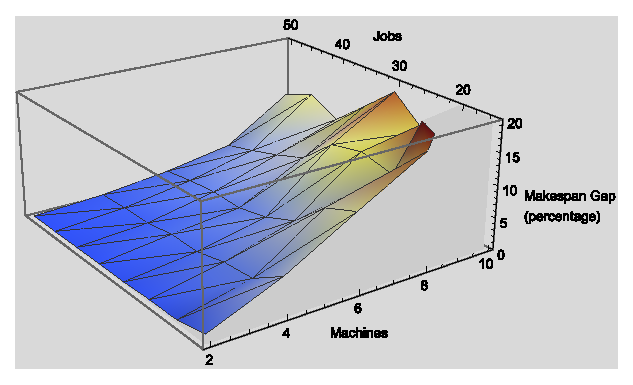
\includegraphics[width=.95\linewidth,height=.7\linewidth]{plots/Q1cRandomMakespangapk=1.eps}};
  \caption{}
  \label{fig:Q1cSFig1}
\end{subfigure}
\begin{subfigure}{.45\textwidth}
  \centering
  \tikz[remember picture]\node[inner sep=0pt,outer sep=0pt] (rates2){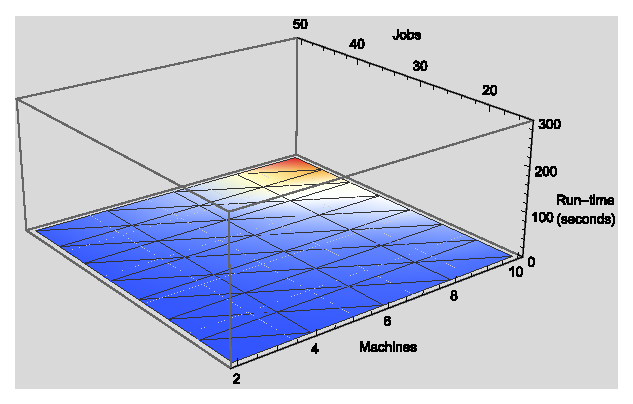
\includegraphics[width=.95\linewidth,height=.7\linewidth]{plots/Q1cRandomRuntimek=1.eps}};
    \caption{}
    \label{fig:Q1cSFig2}
\end{subfigure}
\\
\centering
\begin{subfigure}{.05\textwidth}
\rotatebox[origin=tl]{0}{$k=2$}
\label{fig:Q1cSFig0}
\end{subfigure}
\begin{subfigure}{.45\textwidth}
  \centering
 \tikz[remember picture]\node[inner sep=0pt,outer sep=0pt] (rates3){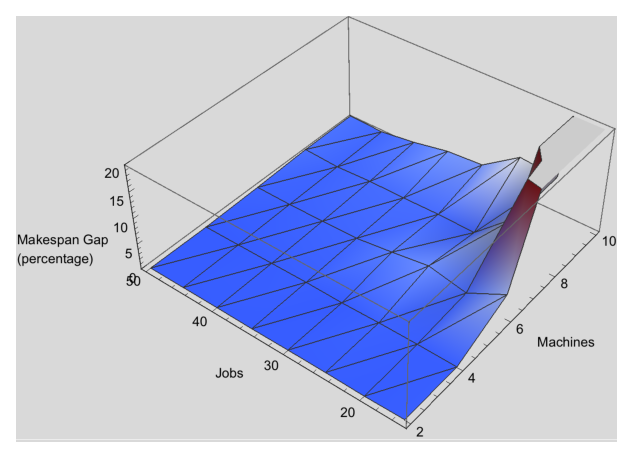
\includegraphics[width=.95\linewidth,height=.7\linewidth]{plots/Q1cRandomMakespangapk=2.eps}};
   \caption{}
  \label{fig:Q1cSFig3}
\end{subfigure}
\begin{subfigure}{.45\textwidth}
  \centering
  \tikz[remember picture]\node[inner sep=0pt,outer sep=0pt] (rates4){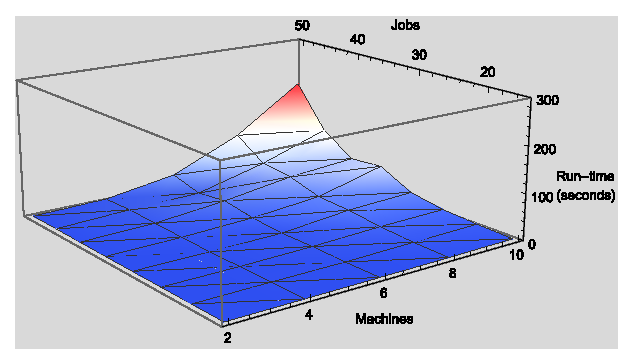
\includegraphics[width=.95\linewidth,height=.7\linewidth]{plots/Q1cRandomRuntimek=2.eps}};
  \caption{}
  \label{fig:Q1cSFig4}
\end{subfigure}
\\
\centering
\begin{subfigure}{.05\textwidth}
\rotatebox[origin=tl]{0}{$k=3$}
\label{fig:Q1cSFig0}
\end{subfigure}
\begin{subfigure}{.45\textwidth}
  \centering
 \tikz[remember picture]\node[inner sep=0pt,outer sep=0pt] (rates3){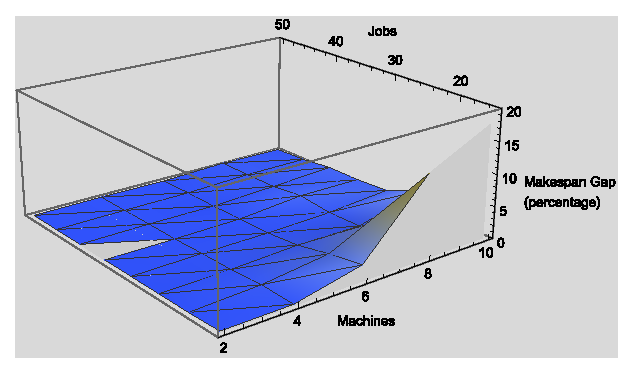
\includegraphics[width=.95\linewidth,height=.7\linewidth]{plots/Q1cRandomMakespangapk=3.eps}};
   \caption{}
  \label{fig:Q1cSFig5}
\end{subfigure}
\begin{subfigure}{.45\textwidth}
  \centering
  \tikz[remember picture]\node[inner sep=0pt,outer sep=0pt] (rates4){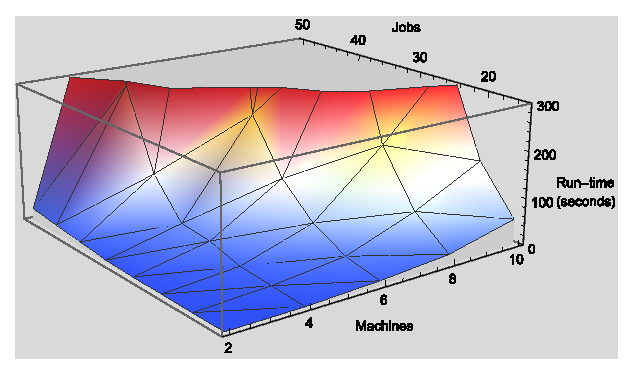
\includegraphics[width=.95\linewidth,height=.7\linewidth]{plots/Q1cRandomRuntimek=3.eps}};
  \caption{}
  \label{fig:Q1cSFig6}
\end{subfigure}
\caption{\textbf{GLS Experiments: $k=1,2,3$, using a random initial solution.}}
\label{fig:Q1c}

\end{figure}

\section*{GLS 1.d}
We perform an experimental study to test the performance of the GLS algorithm, using $k=2$. We test for $n=10,20,30,40,50,60,70,80,90,100$ and $m=2,4,6,8,10$. \\

For each combination of $n$, $m$ and $k$, we generate 10 instances of MS. For each instance, we randomly select the processing times $p_i$, for $i=1,...,n$, uniformly distributed between 1 and 100. Each instance is generated with a different random seed. \\

We now also use different initial solutions; before starting the GLS algorithm, we need to find an initial, feasible solution for the instance. We do this by randomly putting the jobs in any machine ('random'), or by using the greedy makespan algorithm ('GMS'). The GMS works by first sorting the jobs by non-increasing processing time, assigning the $m$ largest jobs each to a different machine, and assigning the remaining jobs to the least loaded machine. \\

We consider a `reasonable' runtime to be approximately 5 minutes. The averaged results of 10 realizations per $n$, $m$, and $k$ are presented in Table \ref{tab:Q1d} and Figure \ref{fig:Q1d}. In Figure \ref{fig:Q1d}, only makespan gap values between 0 and 20 \% are plotted, and run time values between 0 and 300 s (5 minutes). \\

From Table \ref{tab:Q1dmakespangapRandom}, we can calculate that the average makespan gap over all $n$ and $m$ for the random initial solution is 4.09 \%. In Table \ref{tab:Q1dmakespangapGMS}, the average makespan gap over all $n$ and $m$ for the random initial solution is 4.11 \%. In Table \ref{tab:Q1druntimeRandom}, the average run time over all $n$ and $m$ for the GMS initial solution is 176.74 s. In Table \ref{tab:Q1druntimeGMS}, the average run time over all $n$ and $m$ for the GMS initial solution is 171.04 s. Hence, the random initial solution and the GMS initial solution give similar results. \color{red} WHY \color{black} Later we will also use these two initial solutions when testing VDS and our heuristic.


\begin{table}
\begin{center}
{\Large \bf GLS experiments}
\end{center}
\begin{center}
{\large Random initial solution}
\end{center}
\raggedright
%\caption{k=1 \color{red} AND SAME TABLES FOR K=2 AND K=3, PREFER NEXT TO EACH OTHER \color{black}}
\begin{subtable}{0.48\textwidth}
\caption[Makespan gap]{Makespan gap}
%\renewcommand\arraystretch{1.3}
\renewcommand\tabcolsep{1pt}
\centering
\scriptsize
\begin{tabular}{l|*{11}{c}}
\backslashbox{m}{n} & 10 & 20 & 30 & 40 & 50 & 60 & 70 & 80 & 90 & 100 \\
\hline
2& 0.56&	0.06&	0.05&	0&	0.02&	0.02&	0.02&	0.01&	0.02&	0.01 \\
4& 6.23&	0.54&	0.22&	0.10&	0.10&	0.05&	0.02&	0.04&	0.02&	0.02 \\
6& 17.52&	1.05&	0.36&	0.29&	0.15&	0.15&	0.07&	0.09&	0.10&	0.07 \\
8& 66.76&	5.64&	1.12&	0.50&	0.27&	0.37&	0.17&	0.12&	0.14&	0.15 \\
10& 86.32&	9.86&	2.13&	0.87&	0.64&	0.33&	0.26&	0.32&	0.27&	0.20
\end{tabular}
\label{tab:Q1dmakespangapRandom}
\end{subtable}
\begin{subtable}{0.48\textwidth}
\centering
\caption[Run time]{Run time}
%\renewcommand\arraystretch{1.3}
\renewcommand\tabcolsep{1pt}
\centering
\scriptsize
\begin{tabular}{l|*{11}{c}}
\backslashbox{m}{n} & 10 & 20 & 30 & 40 & 50 & 60 & 70 & 80 & 90 & 100 \\
\hline
2& 0.00&	0.02&	0.11&	0.19&	0.54&	1.78&	4.51&	5.66&	7.93&	14.52 \\
4& 0.04&	0.23&	0.84&	2.22&	4.81&	8.02&	19.77&	62.60&	82.57&	131.87 \\
6& 0.78&	0.80&	3.09&	9.10&	25.45&	51.87&	116.10&	206.22&	322.23&	456.87 \\
8& 10.07&	5.73&	13.29&	21.49&	61.11&	97.83&	198.89&	427.29&	640.75&	1117.00 \\
10& 32.48&	23.80&	39.58&	98.76&	185.58&	360.85&	659.68&	533.94&	1154.13&	1614.11
\end{tabular}
\label{tab:Q1druntimeRandom}
\end{subtable}
\begin{center}
\vspace{0.6cm}
{\large GMS initial solution}
\end{center}
\begin{subtable}{0.48\textwidth}
\centering
\caption[Makespan gap]{Makespan gap}
%\renewcommand\arraystretch{1.3}
\renewcommand\tabcolsep{1pt}
\centering
\scriptsize
\begin{tabular}{l|*{11}{c}}
\backslashbox{m}{n} & 10 & 20 & 30 & 40 & 50 & 60 & 70 & 80 & 90 & 100 \\
\hline
2& 0.52&	0.06&	0.05&	0&	0.02&	0.02&	0.02&	0.01&	0.02&	0.01 \\
4& 6.44&	0.35&	0.16&	0.08&	0.07&	0.03&	0.02&	0.04&	0.02&	0.02 \\
6& 17.52&	1.54&	0.57&	0.29&	0.17&	0.07&	0.10&	0.10&	0.07&	0.07 \\
8& 66.76&	6.27&	0.85&	0.57&	0.36&	0.27&	0.14&	0.12&	0.09&	0.09 \\
10& 86.32&	9.75&	2.33&	1.07&	0.45&	0.36&	0.26&	0.34&	0.21&	0.17
\end{tabular}
\label{tab:Q1dmakespangapGMS}
\end{subtable}
\begin{subtable}{0.48\textwidth}
\centering
\caption[Run time]{Run time}
%\renewcommand\arraystretch{1.3}
\renewcommand\tabcolsep{1pt}
\centering
\scriptsize
\begin{tabular}{l|*{11}{c}}
\backslashbox{m}{n} & 10 & 20 & 30 & 40 & 50 & 60 & 70 & 80 & 90 & 100 \\
\hline
2& 0.00&	0.02&	0.11&	0.17&	1.17&	0.92&	3.56&	6.89&	14.87&	11.88 \\
4& 0.03&	0.16&	0.56&	1.9&	3.43&	7.78&	10.23&	58.41&	60.2&	153.82 \\
6& 0.88&	1.12&	3.21&	6.83&	20.65&	47&	99.3&	166.63&	203.52&	209.51 \\
8& 5.42&	8.8&	23.13&	15.65&	38.21&	62.5&	175.91&	530.53&	602.13&	1157.53 \\
10& 23.73&	35.67&	37.07&	84.23&	167.81&	399.51&	345.57&	697.98&	1457.24&	1588.73
\end{tabular}
\label{tab:Q1druntimeGMS}
\end{subtable}

\caption{Experiments GLS: k=2, using random and GMS initial solution. The makespan gap is given in \% and the run time in seconds.}
\label{tab:Q1d}
\end{table}







\begin{figure}
\begin{center}
{\Large \bf GLS experiments}
\end{center}
\begin{subfigure}{.5\textwidth}
  \centering
  \tikz[remember picture]\node[inner sep=0pt,outer sep=0pt] (rates1){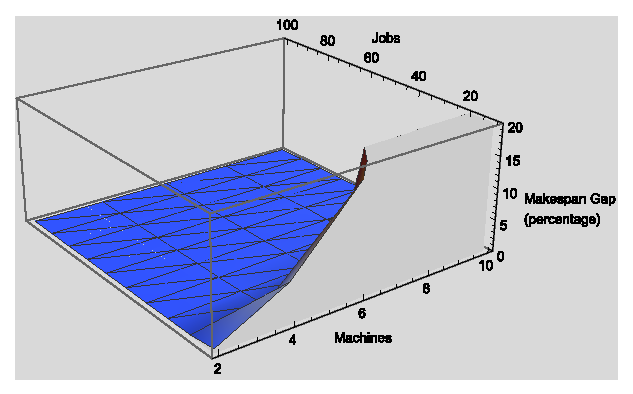
\includegraphics[width=.95\linewidth,height=.7\linewidth]{plots/Q1dRandomMakespanGap.eps}};
  \caption{Random}
  \label{fig:Q1dSFig1}
  \vspace{1cm}
\end{subfigure}%
\begin{subfigure}{.5\textwidth}
  \centering
  \tikz[remember picture]\node[inner sep=0pt,outer sep=0pt] (rates2){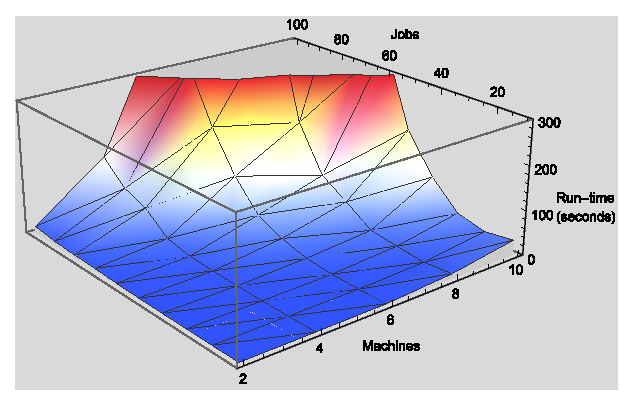
\includegraphics[width=.95\linewidth,height=.7\linewidth]{plots/Q1dRandomRunTime.eps}};
    \caption{Random}
    \label{fig:Q1dSFig2}
    \vspace{1cm}
\end{subfigure}
\begin{subfigure}{.5\textwidth}
  \centering
 \tikz[remember picture]\node[inner sep=0pt,outer sep=0pt] (rates3){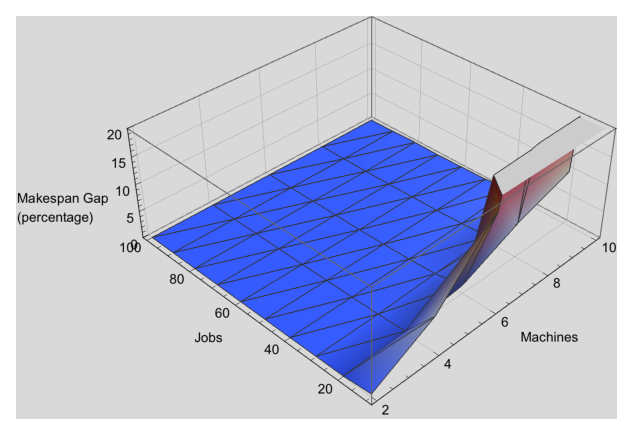
\includegraphics[width=.95\linewidth,height=.7\linewidth]{plots/Q1dGMSMakespanGap.eps}};
   \caption{GMS}
  \label{fig:Q1dSFig3}
\end{subfigure}
\begin{subfigure}{.5\textwidth}
  \centering
  \tikz[remember picture]\node[inner sep=0pt,outer sep=0pt] (rates4){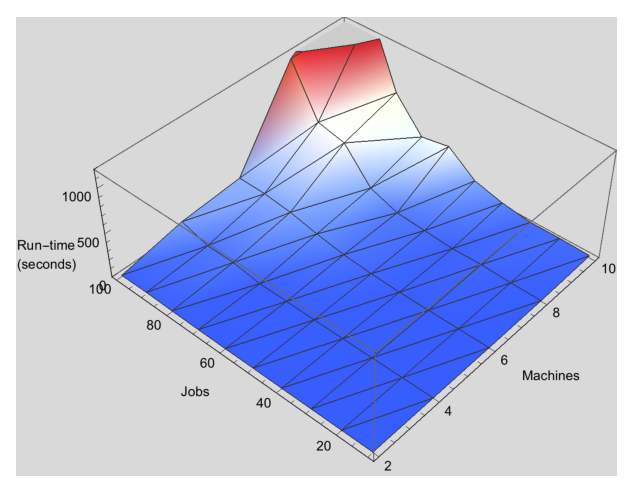
\includegraphics[width=.95\linewidth,height=.7\linewidth]{plots/Q1dGMSRunTime.eps}};
  \caption{GMS}
  \label{fig:Q1dSFig4}
\end{subfigure}
\caption[Experiments GLS: Random and GMS]{\textbf{Experiments GLS: k=2, using random and GMS initial solution.} \small (a) and (b) display the makespan gap (in percentage) and the run time (in seconds), using a random initial solution. (c) and (d) show the makespan gap (in percentage) and the run time (in seconds), using the GMS initial solution. We only plot makespan gap values between 0 and 20 \%, and run time values between 0 and 300 s. }
\label{fig:Q1d}

\end{figure}










\newpage













\section{Variable Depth Search Algorithm for MS}

\section*{VDS 2.a}
\textbf{Pseudo-code for VDS}\\
We begin with an input instance $I = (p_1,p_2,...,p_n,m)$ of the Makespan Scheduling problem. Recall that, during implementation, we use a list $\xi = [\xi_1,\xi_2,...,\xi_n]$ of length $n$, to represent a solution.

\begin{enumerate}
\item Generate an initial feasible solution $\xi = \{\xi_1,\xi_2,...,\xi_n\}$ \color{red} MENTION HOW \color{black}
\item $\textnormal{IMPROVEMENT} := \textnormal{TRUE}$
\item[] $\textnormal{EXCHANGE} := \{1,2,...,n\}$
\item[] $J=0$, $\alpha_J := \xi$
\item \textbf{while} $\textnormal{IMPROVEMENT} = \textnormal{TRUE}$ \textbf{do}
\begin{enumerate}
\item \textbf{while} $\textnormal{EXCHANGE} \neq \emptyset$ \textbf{do}
\begin{enumerate}
\item $J := J+1$
\item $\alpha_J := findBestNeighbour(I,\alpha_{J-1},k,\text{ True, EXCHANGE})$
%the best neighbour in the $k$-neighbourhood of $\alpha_{J-1}$. We define \textit{gain}$(\alpha_{J-1}, \delta) = \textnormal{makespan}(\alpha_{J-1}) - \textnormal{makespan}(\delta)$. Hence, the best neighbour $\alpha_J$ is defined such that \\ \textit{gain}$(\alpha_{J-1},\alpha_J) = $max$\{$\textit{gain}$(\alpha_{J-1},\delta) | \delta \in \textnormal{Neigh}_k(\alpha_{J-1}) - \{\alpha_{J-1} \}$ and $\delta$ differs from $\alpha_{J-1}$ in the parameters of $\textnormal{EXCHANGE}$ only $\}$.
\item $\textnormal{EXCHANGE} := \textnormal{EXCHANGE} - \{\text{jobs whose machines changed in the transition}$\\
\hspace*{6cm} from $\alpha_{J-1} \text{ to } \alpha_{J}\} $
%\item $\textnormal{EXCHANGE} := \textnormal{EXCHANGE} - \{ \textnormal{the parameters in which } \alpha_J \textnormal{ and } \alpha_{J-1} \textnormal{ differ } \}$ (i.e., we remove the job index for which the machine has been changed from $\textnormal{EXCHANGE}$).
\end{enumerate}
\item[] \textbf{end while}
\item Compute \textit{gain}$(\xi,\alpha_i) = \textnormal{makespan}(\xi) - \textnormal{makespan}(\alpha_i)$, for $i=1,...,J$
\item Compute $l \in \{1,...,J\}$ such that \\ \textit{gain}$(\xi,\alpha_l) = \textnormal{max}\{$\textit{gain}$(\xi,\alpha_i) \> | i \in \{1,2,...,J\} \}$
\item \textbf{if} \textit{gain}$(\xi,\alpha_l) > 0$ \textbf{then}
\begin{enumerate}
\item[] $\xi:=\alpha_l$
\item[] $\textnormal{EXCHANGE} := \{1,2,...,n\}$
\end{enumerate}
\item[] \textbf{else}
\begin{enumerate}
\item[] $\textnormal{IMPROVEMENT} := \textnormal{FALSE}$
\end{enumerate}
\end{enumerate}
\item[] \textbf{end while}
\item \textbf{output}$(\alpha)$
\end{enumerate}

\textbf{Neighbourhood function and satisfaction of conditions in Section 3.6.2 of the textbook} \\
Our neighbourhood function, \textit{findBestNeighbour} (step (3)(a)(ii)), returns a solution which can be reached from the input solution in at most $k$ jumps. It does so by systematically iterating through all neighbours and updating the solution if a better neighbour is found. Finding the best neighbour of a feasible solution, $\alpha_i$ is equivalent to finding a feasible solution, $\alpha_{i+1}$, which is such that $gain(\alpha_i,\alpha_{i+1})=\max\{gain(\alpha_i,\delta) | \delta\in Neigh(\alpha_i)\}$. \textcolor{red}{Obvious or explain further?} Thus condition (ii)(a) in Section 3.6.2 of the textbook is satisfied.\\

In order to satisfy the conditions (i) and (ii)(b), we have included two special input arguments to the \textit{findBestNeighbour} method:
\begin{enumerate}
\item \textit{differentSolRequired} is a Boolean parameter, which indicates whether we require a neighbour which differs by at least one $\xi_i$ to the original solution. This is set to be True for the VDS algorithm (whereas for the GLS algorithm, we set it to False). The function does not update the best neighbour if the neighbour is the same as the input solution. The implementation of this parameter ensures that the final feasible solution has all jobs assigned to a different machine to the original solution. Thus condition (i) is satisfied.
\item \textit{jobsToConsider} is a list representing the jobs whose assigned machine we are allowed to change. The \textit{findBestNeighbour} method only iterates over the jobs in this list in its search for the best neighbour, thus returning a solution which is such that any jobs not in the list stay on their original machine. In the VDS algorithm, the input argument is the EXCHANGE list. Thus, at each iteration of the while loop in step (), we obtain a neighbour which differs from the previous solution in the parameters of EXCHANGE only. This list is initialised as the set of all jobs, and is updated at each iteration of the while loop in step () by removing any jobs that were changed. This procedure is continued until there remain no jobs to be changed, and condition (ii)(b) is thus satisfied.
\end{enumerate}

\section*{VDS 2.b}
We use Python to implement the \emph{Variable Depth Search}. See attached.

\section*{VDS 2.c}
We perform an experimental study for VDS using the same instances that were generated for part 1(d)...

\newpage
\section{Simulated Annealing Algorithm for MS}

The heuristic we chose to implement is simulated annealing. In this section, we present pseudocode for the algorithm, as well as details about the generation of the initial value of the temperature. We also present experimental results for the same test instances used in parts 1(d) and 2(c). Finally, we conclude with a comparison to the performance of the simulated annealing heuristic to the performance of the GLS and VDS algorithms.

\subsection*{Simulated Annealing Algorithm Pseudocode}
In our algorithm, we make a slight modification to keep track of the best solution found by the algorithm. This is compared to the final solution found by the simulated annealing algorithm. We do this in order to avoid the algorithm returning a worse solution than one previously found. \\

We again use the GMS algorithm (see section \ref{}) to generate an initial feasible solution. \\

\emph{Input}: An input instance $I = (p_1,p_2,...,p_n,m)$ of the Makespan Scheduling problem.
\begin{enumerate}
\item Generate an initial feasible solution $\xi = \{\xi_1,\xi_2,...,\xi_n\}$, using GMS. \\
$T$ = getInitialTemp($I, k, \chi_0, S, p, \epsilon$)
\item $I := 0$ \\
$best:=\xi$
\item\textbf{while} $T>0$ \textbf{do}
\begin{enumerate}
\item \textbf{begin} Randomly select a neighbour $\beta\in Neigh_x(\alpha)$
\item \textbf{if} makespan($\beta$) $\leq$ makespan($\alpha$) \textbf{then}
\begin{enumerate}
\item $\alpha:=\beta$
\end{enumerate}
\item[] \textbf{else}
\begin{enumerate}
\item Generate a random number $r$ uniformly in the range $(0,1)$
\item \textbf{if} $r<e^{-\frac{\text{makespan}(\alpha)-\text{makespan}(\beta)}{T}}$ \textbf{then}
\begin{enumerate}
\item[] $\alpha:=\beta$
\end{enumerate}
\end{enumerate}
\item \textbf{if}
$\text{makespan}(\alpha) < \text{makespan}(best)$ \textbf{then}
\begin{enumerate}
\item[] $best:=\alpha$
\end{enumerate}
\item $I:=I+1$
\item $T:=\text{reduceTemperature}(T_0,I)$
\end{enumerate}
\item[] \textbf{end while}
\item \textbf{if} $\text{makespan}(\alpha) < \text{makespan}(best)$ \\
\indent \textbf{output}$(\alpha)$ \\
\textbf{else} \\
\indent \textbf{output}$(best)$
\end{enumerate}

\subsection*{Choice of the Initial Temperature: getInitialTemp}
Since the performance of the algorithm varies greatly depending on the initial value of the temperature, we follow the work of Ben-Ameur [\ref{}] to generate an initial temperature. The algorithm produces a value which is based on ... . The pseudocode is as follows.\\

\textbf{Ben-Ameur algorithm for computing the initial temperature}\\
\emph{Input:}
\begin{itemize}
  \item The input instance $I=(p_1,...,p_n,m)$
  \item $k$ exchange value
  \item The desired acceptance probability (?) $\chi_0$
  \item The number of random transitions to generate $S$
  \item $p$ ?
\end{itemize}
\begin{enumerate}
  \item Generate a set, $\mathcal{S}$, of size $S$, of random positive transitions and store the makespan values in $E_{max}$ and $E_{min}$.
  \item $T= ?$
  \item[] Compute $\chi(T):=\frac{\displaystyle\sum\limits_{t\in \mathcal{S}} e^\frac{E_{{max}_{t}}}{T_n}}{\displaystyle\sum\limits_{t\in \mathcal{S}} e^\frac{E_{{min}_{t}}}{T_n}}$
  \item \textbf{while} $|\chi(T)-\chi_0|>\epsilon$ \textbf{do}
  \begin{enumerate}
    \item $T:=T\cdot(\frac{\ln()}{\ln()})^{\frac{1}{p}}$
    \item Compute $\chi(T)$
  \end{enumerate}
  \item \textbf{output} $T$
\end{enumerate}


\subsection*{Choice of the Temperature Reduction Function: reduceTemperature}

We consider several options for the cooling schedule. All are functions, $f$, of the initial temperature, $T_0$, and the iteration number, $I$. \\

\textbf{Exponential multiplicative cooling}
\begin{flalign*}
& f_1(T_0,I)=T_0\cdot \mu^I & \\
& \text{where we set } \mu=0.8. &
\end{flalign*}

\textbf{Simple exponential cooling}
\begin{flalign*}
f_2(T_0,I)=T_0 - I &&
\end{flalign*}

\textbf{Linear multiplicative cooling}
\begin{flalign*}
f_3(T_0,I)=\frac{1}{1+I}\cdot T_0 &&
\end{flalign*}

\textbf{Quadratic multiplicative cooling}
\begin{flalign*}
f_4(T_0,I)=\frac{1}{1+I^2}\cdot T_0 &&
\end{flalign*}

\subsection*{Experimental Study}

\end{document}
